\section{Arjun Yuda Firwanda}

\subsection {Fungsi File CSV, Sejarah dan Contoh}
\begin{itemize}
    \item Fungsi CSV (Comma Separated Values) merupakan format file dalam bahasa pemrogaraman python. CSV adalah file yang berextensi.
    \item File CSV merupakan file khusus yang dapat menyimpan informasi di dalam kolom. CSV memudahkan untuk memindahkan dari satu program ke program y .  Ketika teks dan angka disimpan dalam file CSV, mudah untuk memindahkannya dari satu program ke program lainnya.
    \item Contoh CSV, Microsoft Exel menggunakan format binner atau Binnary Interchange (BIIF). Microsoft merilis office system 2007 dengan format xml. Microsoft Exel juga mendukung format CSV, Dbase File (DBF), Symbolic Link (SYLK), Format Interchange Data (DIF).
\end{itemize}

\subsection {Aplikasi apa saja yang dapat menciptakan file csv}
\begin{itemize}
    \item Text Editor seperti Notepad++, Sublime, Visual Studio Code, Atom.
    \item Program Spreedsheet seperti, Microsoft Exel, Google Spreadshare, LibreOffice.
\end{itemize}

\subsection {Cara Menulis dan membaca file CSV di Exel atau Spreadsheet}
Cara menulisnya paling atassebagai headernya, untuk mepermudah membedakan data. Baris kedua dan seterusnya itu untuk data itu sendiri. Setelah dibuat kemudian di save as dan pilih format CSV. Dan untuk membuka file yang telah dibuat cukup double klik.

\subsection {Jelaskan Library CSV}
Library CSV dibuat untuk memudahkan mengolah data dan mempermudah untuk melakukan export dan import file csv.

\subsection {Jelaskan Library Pandas}
Library Pandas dibuat agar bahasa pemograman python bisa bersaing R dan matlab, yang digunakan untuk mengolah banyak data , keperluan big data, data mining data science.

\subsection {Jelaskan fungsi-fungsi yang terdapat pada library CSV}
\begin{itemize}
    \item Membaca File, fungsi pembacaan file output yang berupa list sebagai hasilnya.
    \item Menulis File, fungsi menulis file pada csv utnuk menyederhanakan contoh data mahasiswa yang terdiri field yaitu nama, npm, kelas. Dan menyimpan hasilnya dengan format datamhs.csv. Kolom atas sebagai headernya, dan kolom kedua dan seterusnya sebagai datanya.
\end{itemize}

\subsection {Jelaskan fungsi-fungsi yang terdapat pada library Pandas}
Fungsi pada library pandas juga hampir sama dengan library csv. Perbedaanya ialah library pandas penulisannya lebih sederhana dan lebih rapih.


\section{Dwi Yulianingsih}
\subsection{Soal 1}
\begin{enumerate}
\subsection{Soal 1}
 CSV (Comma Separated Value) adalah format basis data sederhana yang dimana setiap record yang ada dipisahkan dengan tanda koma (,) atau titik koma (;). Format data file csv dapat diolah dengan berbagai text editor dengan mudah. Anda tidak perlu (dan Anda tidak akan) membuat pengurai CSV Anda sendiri dari awal. Ada beberapa perpustakaan yang dapat diterima yang dapat Anda gunakan. Pustaka csv Python akan berfungsi untuk sebagian besar kasus. Jika pekerjaan Anda memerlukan banyak data atau analisis numerik, panda library juga memiliki kemampuan penguraian CSV, yang seharusnya menangani sisanya. Dalam bahasa pemrograman Python telah disediakan modul csv yang khusus untuk mengolah data berformat csv.  Untuk memanipulasi data csv dengan python tentunya yang pertama dilakukan adalah mengimport modul csv dengan perintah import csv. File CSV biasanya dibuat oleh program yang menangani sejumlah besar data. Mereka adalah cara yang nyaman untuk mengekspor data dari spreadsheet dan basis data serta mengimpor atau menggunakannya dalam program lain. Misalnya, Anda dapat mengekspor hasil program penambangan data ke file CSV dan kemudian mengimpornya ke dalam spreadsheet untuk menganalisis data, menghasilkan grafik untuk presentasi, atau menyiapkan laporan untuk publikasi. Contoh nya adalah sebagai berikut :

 \lstinputlisting[firstline=8, lastline=20]{src/4/1174009/dudul.py}

\subsection{Soal 2}
 Ada beberapa aplikasi yang dapat menciptakan file dengan format csv diantaranya google sheet, number di MacOS dan microsoft excel.

\subsection{Soal 3}
 Cara membuat file csv di excel cukup mudah yaitu :
\begin{itemize}
	\item Buat foldernya
	\item Pilih save as
	\item pilih file dengan format csv
\end{itemize}
Cara membaca file di csv :
\begin{itemize}
	\item Klik data - get external data - form text
	\item Akan muncul Text Import Wizard, arahkan pada file csv yang ingin anda buka lalu Open.
	\item Setelah File terbuka, akan muncul Text Import Wizard.
	\item Pilih Delimited, Kemudian Next (Di sini, bisa juga menentukan baris awal yang akan di import)
	\item Centrang pada Tab dan Comma (Atau sesuai pengaturan File Anda) lalu Next.
	\item Atur Format data pada tiap kolom yang tampil dan klik Finish
\end{itemize}

\subsection{Soal 4}
 CSV muncul untuk memudahkan data science dan analis karena dinilai terdapat banyak kemudahan yang didapat. CSV dapat dimaksimalkan jika dipaduka dengan python karena python adalah bahasa pemrograman yang support ke banyak library termasuk csv. Maka karena itulah perpaduan python dan csv seringkali digunakan oleh perusahaan-perushaan besar dalam mengolah datanya.

\subsection{Soal 5}
Pandas merupakan tool yang dapat digunakan sebagai alat analisis data dan struktur untuk bahasa pemrograman Python. Pandas dapat mengolah data dengan mudah, salah satu fitur yang ada dalam pandas adalah Dataframe. Fitur dataframe dapat membaca sebuah file dan menjadikannya tabble, juga dapat mengolah suatu data dengan menggunakan operasi seperti join, group by dan teknik lainnya yang terdapat pada SQL. Dalam hal ini pandas tidak jauh beda dengan csv yaitu memiliki keunggulan dalam pengolahan data-data besar dan dapat disupport dengan baik dengan python walaupun mengimport data dalam jumlah banyak.

\subsection{Soal 6}
 Library csv mempunyai keunggulan dibandingkan format data lainnya adalah soal kompatibilitas. File csv dapat digunakan, diolah, diekspor/impor, dan dimodifikasi menggunakan berbagai macam perangkat lunak dan bahasa pemrograman. Pada library csv mempunyai fungsi import dan eksport data yang baik dan bisa digunakan dalam jumlah besar.

\subsection{Soal 7}
pandas menyediakan beragam fungsi operasi untuk mengolah data. Contoh jika menggunakan series bisa mencari nilai max, min, dan mean secara langsung, bahkan juga bisa melakukan operasi perpangkatan pada nilai Series secara langsung.
Pandas dapat mengolah suatu data dan mengolahnya seperti join, distinct, group by, agregasi, dan teknik seperti pada SQL. Hanya saja dilakukan pada tabel yang dimuat dari file ke RAM.
\end{enumerate}

\subsection{bukti bebas plagiarisme}
\begin{figure}[H]
\centering
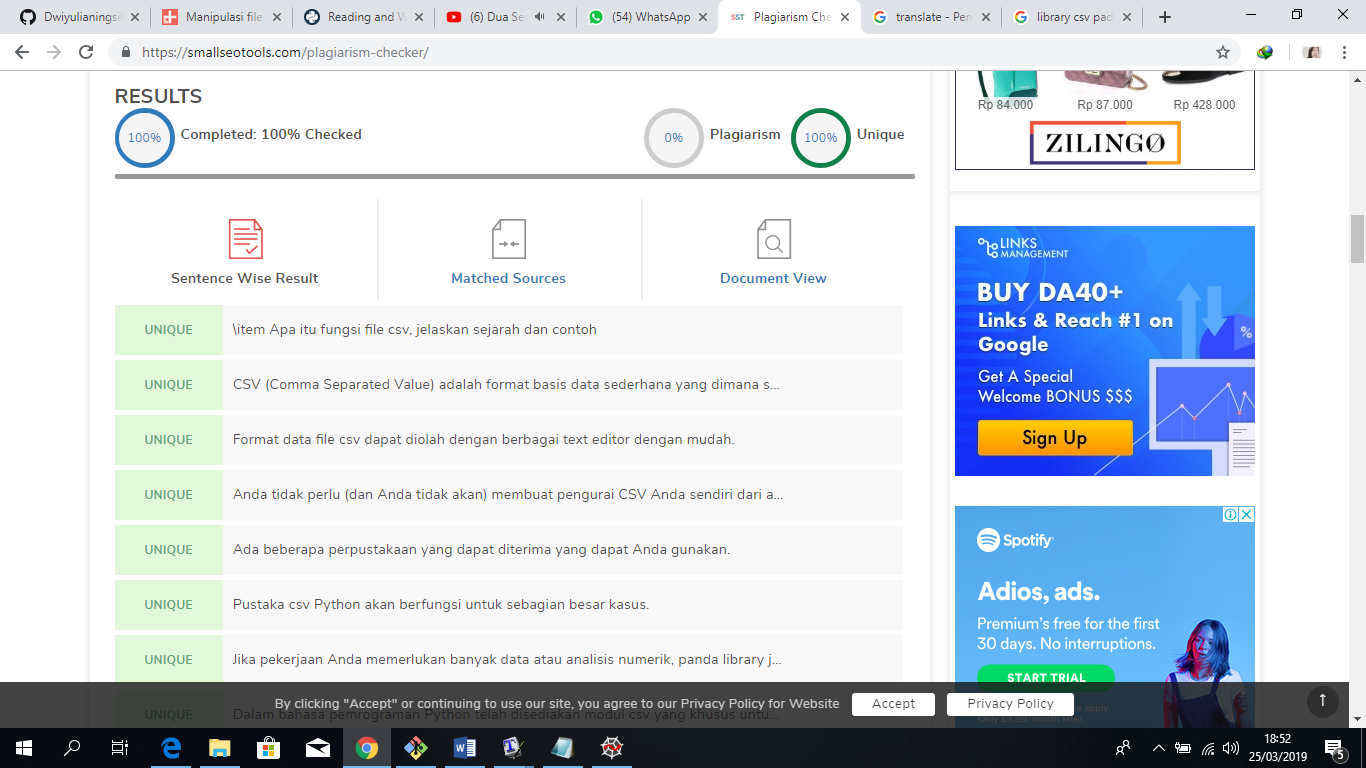
\includegraphics[width=10cm]{figures/4/1174009/yuli.png}
\caption{SS Bebas Plagiarisme}
\label{dwiyul}
\end{figure}


\section{Harun Ar-Rasyid}
\subsection{Soal 1}
File CSV (Nilai Terbatas Koma) adalah jenis file khusus yang dapat Anda buat atau edit di Excel. File CSV menyimpan informasi yang dipisahkan oleh koma, tidak menyimpan informasi dalam kolom. Ketika teks dan angka disimpan dalam file CSV, mudah untuk memindahkannya dari satu program ke program lainnya.
Dari rilis pertama, Excel menggunakan format file biner yang disebut Binary Interchange File Format (BIFF) sebagai format file utamanya. Ini berubah ketika Microsoft merilis Office System 2007 yang memperkenalkan Office Open XML sebagai format file utamanya. Office Open XML adalah file kontainer berbasis XML yang mirip dengan XML Spreadsheets (XMLSS), yang diperkenalkan di Excel 2002. File versi XML tidak bisa menyimpan makro VBA.
Meskipun mendukung format XML baru, Excel 2007 masih mendukung format lama yang masih berbasis BIFF tradisional. Selain itu Microsoft Excel juga mendukung format Comma Separated Values (CSV), DBase File (DBF), SYMbolic LinK (SYLK), Format Interchange Data (DIF) dan banyak format lainnya, termasuk format lembar kerja 1-2 Lotus - 3 (WKS, WK1, WK2, dll.) Dan Quattro Pro.

\subsection{Soal 2}
\begin{itemize}
    \item Texteditor
    Seperti notepad,visual studio code,atom,sublime dan lain sebagainya
    \item Program Spreadsheet
    Seperti excell,google spreadshare,LibreOfficecalc
\end{itemize}

\subsection{Soal 3}
Untuk menulisnya untuk yang paling atas itu kita buat headernya,untuk mepermudah membedakan datanya,dan untuk baris kedua dan seterusnya itu untuk data itu sendiri.
dan setelah di buat kalian save as kemudian pilih format CSV.
dan untuk membukan cukup di double clik file tersebut.

\subsection{Soal 4}
library csv dibuat untuk permudah mengolah data. Dan mempermudah untuk melakukan export dan import file csv itu sendiri

\subsection{Soal 5}
library pandas dibuat agar bahasa pemograman python bisa bersaing R dan matlab, yang digunakan untuk mengolah banyak data , keperluan big data, data mining data science dan sebagainya.

\subsection{Soal 6}
Terdapat 2 fungsi yang bisa digunakan oleh library csv
Pertama,fungsi membaca file csv.
fungsi ini bisa menggunakan list dan dictionary
Dengan list :
\lstinputlisting[firstline=11, lastline=21]{src/4/1174027/teori/c_1174027_csv.py}
Dengan dictionary :
\lstinputlisting[firstline=24, lastline=33]{src/4/1174027/teori/c_1174027_csv.py}
Kedua,fungsi menulis file csv.
\lstinputlisting[firstline=36, lastline=40]{src/4/1174027/teori/c_1174027_csv.py}

\subsection{Soal 7}
Hampir sama dengan library csv,tp library pandas penulisannya lebih sederhana dan terlihat lebih rapih dari pada library csv.
\lstinputlisting[firstline=10, lastline=11]{src/4/1174027/praktek/p_1174027_pandas.py}

\subsection{Bukti Bebas Plagiat}
\begin{figure}[H]
    \centering
    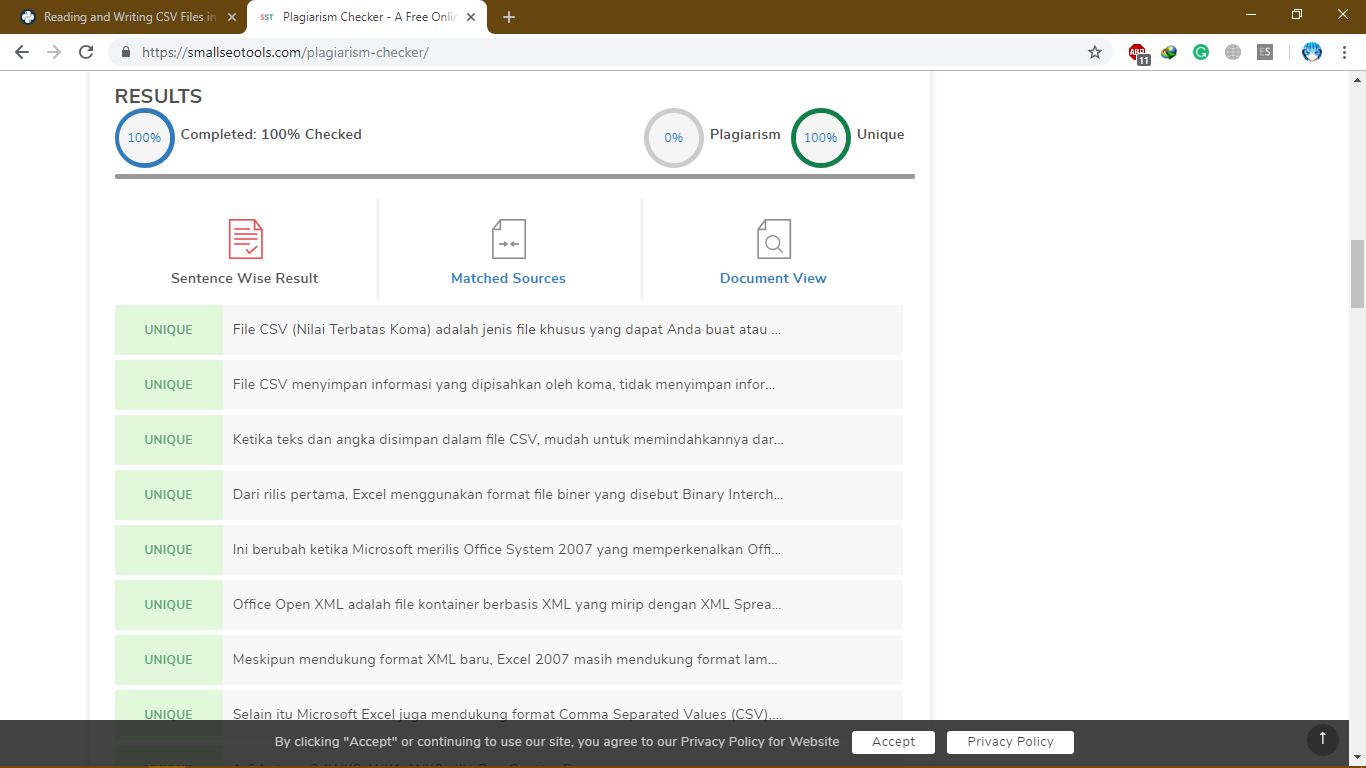
\includegraphics[width=10cm]{figures/4/1174027/teori/harunpla.png}
    \caption{SS Bebas Plagiarisme}
    \label{harun}
\end{figure}

\section{Sri Rahayu}
\subsection{Soal 1}
Isi jawaban soal ke-1

Kalau mau dibikin paragrap \textbf{cukup enter aja}, tidak usah pakai \verb|par| dsb

%\subsection{Soal 2}
%Isi jawaban soal ke-2

%\subsection{Soal 3}
%Isi jawaban soal ke-3

\section{Doli Jonviter}
\subsection{Soal 1}
Isi jawaban soal ke-1

Kalau mau dibikin paragrap \textbf{cukup enter aja}, tidak usah pakai \verb|par| dsb

%\subsection{Soal 2}
%Isi jawaban soal ke-2

%\subsection{Soal 3}
%Isi jawaban soal ke-3

\section{Rahmatul Ridha}
\subsection{Soal 1}
Kerjakan soal berikut ini, masing-masing bernilai 5 untuk hari pertama. Praktek teori penungjang yang dikerjakan dengan deadline besok jam 4 pagi :
\begin{enumerate}
 \item Apa itu fungsi file csv, jelaskan sejarah dan contohnya.
   \begin{itemize}
    \item Apa itu Fungsi file csv

     Format file csv \textit{Comma Separated Values} yaitu suatu format data pada basis data dimana setiap record yang dapat dipisahkan dengan menggunakan tanda koma (`,’) atau juga bisa dengan menggunakan titik koma (`;’) sebagai tanda pemisah antara datu elemen dengan elemen yang lainnya. Selain bahasa programnya yang sederhana, format ini juga dapat dibuka dengan menggunakan berbagai \textit{text-editor} seperti Notepad, Wordpad, dan MS Excel.

     File CSV (nilai berbatas koma) merupakan tipa file khusus yang dapat dibuat atau diedit dengan menggunakan excel. File csv menyimpan informasi yang dapat dipisah oleh koma (,), bukan untuk menyimpan informasi dalam kolom. Saat teks dan angka yang disimpan dalam file csv, dapat memudahkan untuk memindahkannya dari satu program ke program yang lainnya.

    \item Sejarah CSV

     Nilai yang dipisahkan oleh koma adalah format data yang memberi tanggal lebih awal pada komputer pribadi lebih dari satu dekade: kompiler IBM Fortran (level H extended) di bawah OS / 360 mendukungnya pada tahun 1972. Input / output yang diarahkan oleh daftar ("bentuk bebas") didefinisikan dalam FORTRAN 77, disetujui pada tahun 1978. Input yang diarahkan daftar menggunakan koma atau spasi untuk pembatas, sehingga string karakter yang tidak dikutip tidak dapat mengandung koma atau spasi.

     Nama "nilai yang dipisahkan koma" dan singkatan "CSV" digunakan pada tahun 1983. Manual untuk komputer Osborne Executive, yang menggabungkan SuperCalc spreadsheet, mendokumentasikan konvensi kutipan CSV yang memungkinkan string berisi koma yang disematkan, tetapi manual tersebut tidak menentukan konvensi untuk menyematkan tanda kutip dalam string yang dikutip. Daftar nilai yang dipisahkan koma lebih mudah untuk diketik (misalnya ke dalam kartu berlubang) daripada data yang selaras dengan kolom tetap dan cenderung menghasilkan hasil yang salah jika suatu nilai dilubangi satu kolom dari lokasi yang dituju.

     Pada 2014 IETF menerbitkan RFC7111 yang menjelaskan aplikasi fragmen URI ke dokumen CSV. RFC7111 menentukan bagaimana rentang baris, kolom, dan sel dapat dipilih dari dokumen CSV menggunakan indeks posisi. Pada 2015 W3C, dalam upaya meningkatkan CSV dengan semantik formal, mempublikasikan draft rekomendasi pertama untuk standar metadata CSV, yang dimulai sebagai rekomendasi pada bulan Desember tahun yang sama.

     \item Contohnya

       \lstinputlisting[caption = Contoh penggunaan format CSV., firstline=1, lastline=3]{src/4/1144124/Chapter4/teori.csv}
     \end{itemize}

 \item Aplikasi-aplikasi apa saja yang bisa menciptakan file csv ?

       \begin{itemize}
         \item Text editor (Notepat, Wordpad, dan lain-lain)
         \item Spreadsheet (Microsoft Excel)
       \end{itemize}

 \item Jelaskan bagaimana cara menulis dan membaca file csv diexcel atau spreadsheet.

    \textbf{Menulis File CSV}
       \begin{enumerate}
	   \item Buat dokumen baru diexcel.
       \item Tambahkan judul kolom untuk setiap potongan informasi yang ingin dicatat, contohnya npm, nama, kelas. Lalu ketikkn informasi delam kolom yang sesuai.
	   \item Setelah selesai dibuat, file excel yang telah dibuat akan terlihat seperti \ref{CSV}
		
		\begin{figure}[H]	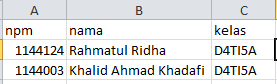
\includegraphics[width=5cm]{figures/4/1144124/Chapter4/1.png}
		\centering
        \caption{Membuat file csv}
        \label{CSV}
		\end{figure}
		
	   \item Kemudian isi kolom `File name' dengan nama file anda dan kolom `Save as type' pilih yang berekstensi .csv \ref{save}.
		\begin{figure}[H] \includegraphics[width=5cm]{figures/4/1144124/Chapter4/2.png}
			\centering
        \caption{Save as Type}
        \label{save}
		\end{figure}

\item Kemudian file yang Anda telah terbuat tadi tersimpan dengan ekstensi .csv. Untuk melihat isi filenya tinggal klik dua kali pada file tersebut \ref{ekstensi}.

		\begin{figure}[H]	\includegraphics[width=5cm]{figures/4/1144124/Chapter4/3.png}
			\centering
        \caption{Perintah ekstensi}
        \label{ekstensi}
		\end{figure}
		
	   \item Lalu tinggal klik `Yes'\ref{lokasipenyimpanan}.
	
		\begin{figure}[H] \includegraphics[width=5cm]{figures/4/1144124/Chapter4/4.png}
		\centering
		\caption{Konfirmasi Penyimpanan}
        \label{lokasipenyimpanan}
        \end{figure}
        \end{enumerate}

   \textbf{Melihat File CSV di Excel atau Spreadsheet}

	 \begin{enumerate}
		\item Pertama klik dua kali pada file yang yang berekstensi CSV\ref{filecsv}.
		
		\begin{figure}[H]	
\includegraphics[width=5cm]{figures/4/1144124/Chapter4/5.png}
		\centering
		\caption{file csv yang telah disave}
        \label{filecsv}
        \end{figure}
		
		\item Kemudian file akan terbuka secara otomatis di aplikasi Excel atau spreadsheet\ref{filecsv1}.
		
		\begin{figure}[H] 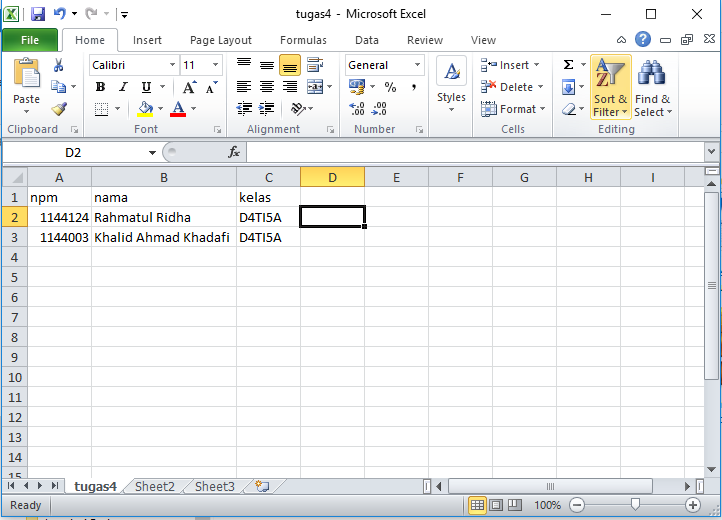
\includegraphics[width=5cm]{figures/4/1144124/Chapter4/6.png}
		\centering
        \caption{file csv pada Excel}
        \label{filecsv1}
		\end{figure}
	 \end{enumerate}

   \item Jelaskan sejarah library csv.

   Format yang disebut CSV \textit{Comma Separated Values} adalah format impor dan ekspor paling umum untuk spreadsheet dan basis data. Format CSV digunakan selama bertahun-tahun sebelum upaya untuk menggambarkan format dengan cara standar di RFC 4180. Kurangnya standar yang didefinisikan dengan baik berarti bahwa perbedaan halus sering ada dalam data yang diproduksi dan dikonsumsi oleh aplikasi yang berbeda. Perbedaan-perbedaan ini dapat membuatnya menjengkelkan untuk memproses file CSV dari berbagai sumber.

   Namun, sementara pembatas dan mengutip karakter bervariasi, format keseluruhan cukup mirip sehingga dimungkinkan untuk menulis satu modul yang dapat secara efisien memanipulasi data seperti itu, menyembunyikan detail membaca dan menulis data dari programmer. Modul csv mengimplementasikan kelas untuk membaca dan menulis data tabular dalam format CSV.

   Hal ini memungkinkan programmer untuk mengatakan, "tulis data ini dalam format yang disukai oleh Excel," atau "baca data dari file ini yang dihasilkan oleh Excel," tanpa mengetahui detail yang tepat dari format CSV yang digunakan oleh Excel. Pemrogram juga dapat menggambarkan format CSV yang dipahami oleh aplikasi lain atau menentukan format CSV tujuan khusus mereka sendiri.

   \item Jelaskan sejarah library Pandas.
   
   Pandas merupakan toolkit yang powerfull sebagai alat untuk analisis data dan struktur pada bahasa pemrograman Python. Dengan menggunakan pandas kita dapat mengolah data dengan mudah, salah satunya yaitu fiturnya adalah Dataframe. Dengan adanya fitur dataframe kita dapat membaca sebuah file dan menjadikannya tabel, kita juga dapat mengolah suatu data dengan menggunakan operasi seperti join, distinct, group by, agregasi, dan teknik lainnya yang terdapat pada SQL. Saat ini banyak format file yang dapat dibaca menggunakan Pandas, seperti file .txt, .csv, .tsv dan lainnya.

   \item Jelaskan fungsi-fungsi yang terdapat dilibrary csv.

       \begin{enumerate}
		\item reader
		
		Fungsi ini digunakan untuk membaca isi file berformat CSV dari list.
		
		\lstinputlisting[caption = Membaca file berformat CSV list., firstline=7, lastline=13]{src/4/1144124/Chapter4/1144124.py}
		
		\item DictReader
		
		Fungsi ini digunakan untuk membaca isi file berformat CSV dari dictionary.
		
		\lstinputlisting[caption =  Membaca file berformat CSV dictionary., firstline=15, lastline=21]{src/4/1144124/Chapter4/1144124.py}
		
		\item write
		
		Fungsi ini digunakan untuk menulis file berformat CSV dari list.
		
		\lstinputlisting[caption =  Menulis file berformat CSV list., firstline=23, lastline=30]{src/4/1144124/Chapter4/1144124.py}
		
		\item DictWrite
		
		Fungsi ini digunakan untuk menulis file berformat CSV dari dictionary.
		
		\lstinputlisting[caption =  Menulis file berformat CSV dictionary., firstline=32, lastline=41]{src/4/1144124/Chapter4/1144124.py}
		
	\end{enumerate}

   \item Jelaskan fungsi-fungsi yang terdapat di library pandas.

       \begin{enumerate}
		\item read\_csv
		
		Fungsi ini digunakan untuk membaca isi file berformat CSV
		
		\lstinputlisting[caption =  Membaca file berformat CSV pandas., firstline=43, lastline=47]{src/4/1144124/Chapter4/1144124.py}
		
		\item to\_csv
		
		Fungsi ini digunakan untuk menulis file berformat CSV
		
		\lstinputlisting[caption =  Menulis file berformat CSV pandas., firstline=49, lastline=53]{src/4/1144124/Chapter4/1144124.py}
		
	\end{enumerate}
   \item Cek plagiarisme

Berikut adalah cek plagiarisme pada teorinya pada \ref{Plagiarisme}

   \begin{figure}[H]
	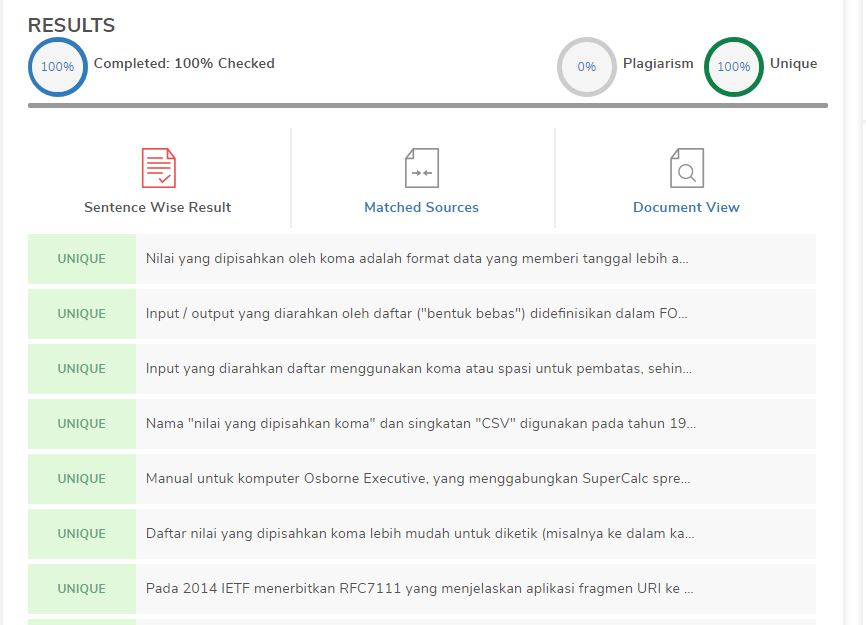
\includegraphics[width=5cm]{figures/4/1144124/Chapter4/Plagiarisme.jpg}
	\centering
    \caption{Plagiarisme}
    \label{Plagiarisme}
    \end{figure}
 \end{enumerate}

\section{Tomy Prawoto}
\subsection{Soal 1}
Isi jawaban soal ke-1

\begin{enumerate}
 \item Apa itu fungsi file csv, jelaskan sejarah dan contohnya.
   \begin{itemize}
    \item Apa itu Fungsi file csv

     Format file csv \textit{Comma Separated Values} yaitu suatu format data pada basis data dimana setiap record yang dapat dipisahkan dengan menggunakan tanda koma (`,’) atau juga bisa dengan menggunakan titik koma (`;’) sebagai tanda pemisah antara datu elemen dengan elemen yang lainnya. Selain bahasa programnya yang sederhana, format ini juga dapat dibuka dengan menggunakan berbagai \textit{text-editor} seperti Notepad, Wordpad, dan MS Excel.

     File CSV (nilai berbatas koma) merupakan tipa file khusus yang dapat dibuat atau diedit dengan menggunakan excel. File csv menyimpan informasi yang dapat dipisah oleh koma (,), bukan untuk menyimpan informasi dalam kolom. Saat teks dan angka yang disimpan dalam file csv, dapat memudahkan untuk memindahkannya dari satu program ke program yang lainnya.

    \item Sejarah CSV

     Nilai yang dipisahkan oleh koma adalah format data yang memberi tanggal lebih awal pada komputer pribadi lebih dari satu dekade: kompiler IBM Fortran (level H extended) di bawah OS / 360 mendukungnya pada tahun 1972. Input / output yang diarahkan oleh daftar ("bentuk bebas") didefinisikan dalam FORTRAN 77, disetujui pada tahun 1978. Input yang diarahkan daftar menggunakan koma atau spasi untuk pembatas, sehingga string karakter yang tidak dikutip tidak dapat mengandung koma atau spasi.

     Nama "nilai yang dipisahkan koma" dan singkatan "CSV" digunakan pada tahun 1983. Manual untuk komputer Osborne Executive, yang menggabungkan SuperCalc spreadsheet, mendokumentasikan konvensi kutipan CSV yang memungkinkan string berisi koma yang disematkan, tetapi manual tersebut tidak menentukan konvensi untuk menyematkan tanda kutip dalam string yang dikutip. Daftar nilai yang dipisahkan koma lebih mudah untuk diketik (misalnya ke dalam kartu berlubang) daripada data yang selaras dengan kolom tetap dan cenderung menghasilkan hasil yang salah jika suatu nilai dilubangi satu kolom dari lokasi yang dituju.

     Pada 2014 IETF menerbitkan RFC7111 yang menjelaskan aplikasi fragmen URI ke dokumen CSV. RFC7111 menentukan bagaimana rentang baris, kolom, dan sel dapat dipilih dari dokumen CSV menggunakan indeks posisi. Pada 2015 W3C, dalam upaya meningkatkan CSV dengan semantik formal, mempublikasikan draft rekomendasi pertama untuk standar metadata CSV, yang dimulai sebagai rekomendasi pada bulan Desember tahun yang sama.

     \item Contohnya

       \lstinputlisting[caption = Contoh penggunaan format CSV., firstline=1, lastline=3]{src/4/1154121/Chapter4/teori.csv}
     \end{itemize}

 \item Aplikasi-aplikasi apa saja yang bisa menciptakan file csv ?

       \begin{itemize}
         \item Text editor (Notepat, Wordpad, dan lain-lain)
         \item Spreadsheet (Microsoft Excel)
       \end{itemize}

 \item Jelaskan bagaimana cara menulis dan membaca file csv diexcel atau spreadsheet.

    \textbf{Menulis File CSV}
       \begin{enumerate}
	   \item Buat dokumen baru diexcel.
       \item Tambahkan judul kolom untuk setiap potongan informasi yang ingin dicatat, contohnya npm, nama, kelas. Lalu ketikkn informasi delam kolom yang sesuai.
	   \item Setelah selesai dibuat, file excel yang telah dibuat akan terlihat seperti \ref{CSV}
		
		\begin{figure}[H]	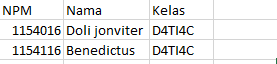
\includegraphics[width=5cm]{figures/4/1154121/1.png}
		\centering
        \caption{Membuat file csv}
        \label{CSV}
		\end{figure}
		
	   \item Kemudian isi kolom `File name' dengan nama file anda dan kolom `Save as type' pilih yang berekstensi .csv \ref{save}.
		\begin{figure}[H] \includegraphics[width=5cm]{figures/4/1154121/2.png}
			\centering
        \caption{Save as Type}
        \label{save}
		\end{figure}

\item Kemudian file yang Anda telah terbuat tadi tersimpan dengan ekstensi .csv. Untuk melihat isi filenya tinggal klik dua kali pada file tersebut \ref{ekstensi}.

		\begin{figure}[H]	\includegraphics[width=5cm]{figures/4/1154121/3.png}
			\centering
        \caption{Perintah ekstensi}
        \label{ekstensi}
		\end{figure}
		
	   \item Lalu tinggal klik `Yes'\ref{lokasipenyimpanan}.
	
		\begin{figure}[H] \includegraphics[width=5cm]{figures/4/1154121/4.png}
		\centering
		\caption{Konfirmasi Penyimpanan}
        \label{lokasipenyimpanan}
        \end{figure}
        \end{enumerate}

   \textbf{Melihat File CSV di Excel atau Spreadsheet}

	 \begin{enumerate}
		\item Pertama klik dua kali pada file yang yang berekstensi CSV\ref{filecsv}.
		
		\begin{figure}[H]	
\includegraphics[width=5cm]{figures/4/1154121/5.png}
		\centering
		\caption{file csv yang telah disave}
        \label{filecsv}
        \end{figure}
		
		\item Kemudian file akan terbuka secara otomatis di aplikasi Excel atau spreadsheet\ref{filecsv1}.
		
		\begin{figure}[H] 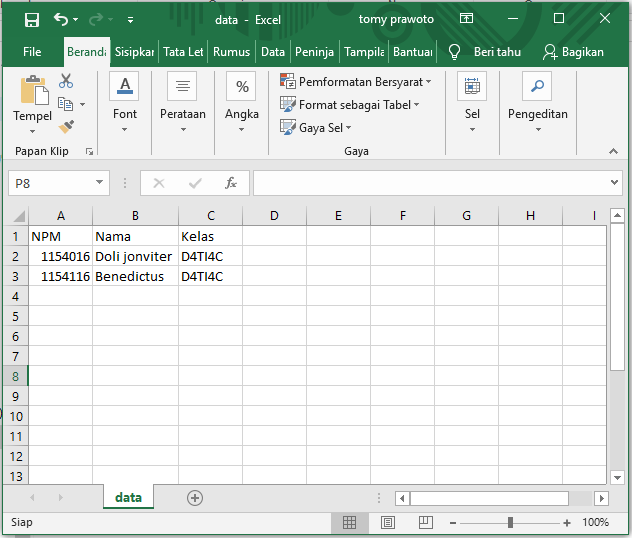
\includegraphics[width=5cm]{figures/4/1154121/6.png}
		\centering
        \caption{file csv pada Excel}
        \label{filecsv1}
		\end{figure}
	 \end{enumerate}

   \item Jelaskan sejarah library csv.

   Format yang disebut CSV \textit{Comma Separated Values} adalah format impor dan ekspor paling umum untuk spreadsheet dan basis data. Format CSV digunakan selama bertahun-tahun sebelum upaya untuk menggambarkan format dengan cara standar di RFC 4180. Kurangnya standar yang didefinisikan dengan baik berarti bahwa perbedaan halus sering ada dalam data yang diproduksi dan dikonsumsi oleh aplikasi yang berbeda. Perbedaan-perbedaan ini dapat membuatnya menjengkelkan untuk memproses file CSV dari berbagai sumber.

   Namun, sementara pembatas dan mengutip karakter bervariasi, format keseluruhan cukup mirip sehingga dimungkinkan untuk menulis satu modul yang dapat secara efisien memanipulasi data seperti itu, menyembunyikan detail membaca dan menulis data dari programmer. Modul csv mengimplementasikan kelas untuk membaca dan menulis data tabular dalam format CSV.

   Hal ini memungkinkan programmer untuk mengatakan, "tulis data ini dalam format yang disukai oleh Excel," atau "baca data dari file ini yang dihasilkan oleh Excel," tanpa mengetahui detail yang tepat dari format CSV yang digunakan oleh Excel. Pemrogram juga dapat menggambarkan format CSV yang dipahami oleh aplikasi lain atau menentukan format CSV tujuan khusus mereka sendiri.

   \item Jelaskan sejarah library Pandas.
   
   Pandas merupakan toolkit yang powerfull sebagai alat untuk analisis data dan struktur pada bahasa pemrograman Python. Dengan menggunakan pandas kita dapat mengolah data dengan mudah, salah satunya yaitu fiturnya adalah Dataframe. Dengan adanya fitur dataframe kita dapat membaca sebuah file dan menjadikannya tabel, kita juga dapat mengolah suatu data dengan menggunakan operasi seperti join, distinct, group by, agregasi, dan teknik lainnya yang terdapat pada SQL. Saat ini banyak format file yang dapat dibaca menggunakan Pandas, seperti file .txt, .csv, .tsv dan lainnya.

   \item Jelaskan fungsi-fungsi yang terdapat dilibrary csv.

       \begin{enumerate}
		\item reader
		
		Fungsi ini digunakan untuk membaca isi file berformat CSV dari list.
		
		\lstinputlisting[caption = Membaca file berformat CSV list., firstline=7, lastline=13]{src/4/1154121/Chapter4/1154121.py}
		
		\item DictReader
		
		Fungsi ini digunakan untuk membaca isi file berformat CSV dari dictionary.
		
		\lstinputlisting[caption =  Membaca file berformat CSV dictionary., firstline=15, lastline=21]{src/4/1154121/Chapter4/1154121.py}
		
		\item write
		
		Fungsi ini digunakan untuk menulis file berformat CSV dari list.
		
		\lstinputlisting[caption =  Menulis file berformat CSV list., firstline=23, lastline=30]{src/4/1154121/Chapter4/1154121.py}
		
		\item DictWrite
		
		Fungsi ini digunakan untuk menulis file berformat CSV dari dictionary.
		
		\lstinputlisting[caption =  Menulis file berformat CSV dictionary., firstline=32, lastline=41]{src/4/1154121/Chapter4/1154121.py}
		
	\end{enumerate}

   \item Jelaskan fungsi-fungsi yang terdapat di library pandas.

       \begin{enumerate}
		\item read\_csv
		
		Fungsi ini digunakan untuk membaca isi file berformat CSV
		
		\lstinputlisting[caption =  Membaca file berformat CSV pandas., firstline=43, lastline=47]{src/4/1154121/Chapter4/1154121.py}
		
		\item to\_csv
		
		Fungsi ini digunakan untuk menulis file berformat CSV
		
		\lstinputlisting[caption =  Menulis file berformat CSV pandas., firstline=49, lastline=53]{src/4/1154121/Chapter4/1154121.py}
		
	\end{enumerate}
 \end{enumerate}

